\section{Experiment}
\label{others}
% Requires: booktabs, amssymb, graphicx, natbib. Figures are in figures/ (regenerate with figures/make_figures.py and figures/make_qualitative.py).

<<E1>> <<E2>> <<E3>>
% 我们在离线位姿估计和闭环飞行两种情境下评估同一个模型。图~\ref{fig:qualitative} 给出定性示例，图~\ref{fig:breakdown} 展示想象精修阶段的作用。实验表明：1）在航拍视图间的位姿估计上，DreamNav 比现有的导航策略、世界模型和视觉表征更准确；2）几何想象让每个位姿参数都比只用粗估计阶段更准确；3）在真实无人机照片上，当基线落在训练范围内时，DreamNav 明显比回归基线更准确。

\begin{table*}[!t]
    \centering
    \caption{<<C1>> <<C2>> <<C1b>>}
    \label{tab:main_result}
    \small
    \setlength{\tabcolsep}{4.2pt}
    \begin{tabular}{l|cccccc|c|ccc}
        \toprule
        & \multicolumn{6}{c|}{MAE $\downarrow$} & SR $\uparrow$ & \multicolumn{3}{c}{Pose AUC $\uparrow$} \\
        Methods & $\Delta x$ (m) & $\Delta y$ (m) & $\Delta z$ (m) & $d$ (m) & $\Delta\theta$ ($^\circ$) & $\Delta\phi$ ($^\circ$) & @1\,m & @5$^\circ$ & @10$^\circ$ & @20$^\circ$ \\
        \midrule
        Constant (zero motion) & 7.45 & 7.45 & 15.40 & 20.32 & 85.81 & 20.02 & 0.0 & 0.2 & 0.6 & 1.3 \\
        \midrule
        AI2-THOR~\citep{7989381} & 7.46 & 7.44 & 15.41 & 19.32 & 85.80 & 18.22 & 0.1 & 0.3 & 0.8 & 1.8 \\
        $\pi_{0.5}$~\citep{intelligence2025pi_} & 9.36 & 9.57 & 19.45 & 7.64 & 80.72 & 4.16 & 8.4 & 0.9 & 2.8 & 6.7 \\
        $\pi_0$-FAST~\citep{pertsch2025fast} & 10.38 & 10.59 & 15.16 & 6.12 & 76.13 & 2.67 & 11.3 & 4.0 & 7.7 & 10.2 \\
        ViNT~\citep{shah2023vint} & 7.46 & 7.46 & 15.44 & 5.92$^\ddagger$ & 51.83 & 11.27 & 10.2$^\ddagger$ & 1.5 & 4.4 & 11.4 \\
        NoMaD~\citep{sridhar2024nomad} & 9.75 & 9.49 & 19.53 & 6.78$^\ddagger$ & 86.19 & 15.93 & 9.2$^\ddagger$ & 0.4 & 1.2 & 3.7 \\
        DINO-WM~\citep{zhou2025dinowm} & 8.92 & 9.06 & 19.29 & 10.23 & 84.59 & 11.09 & 6.2 & 0.4 & 1.4 & 4.3 \\
        Visual Foresight~\citep{ebert2018visual} & 8.80 & 8.67 & 18.64 & 10.30 & 83.09 & 7.97 & 5.7 & 0.5 & 1.9 & 5.6 \\
        DINOv3 ViT-7B~\citep{simeoni2025dinov3} & 7.70 & 7.70 & 14.27 & 13.39 & 86.23 & 4.44 & 2.7 & 0.7 & 2.3 & 5.5 \\
        Sample4Geo~\citep{deuser2023sample4geo} & 8.60 & 8.29 & 15.88 & 10.59 & 85.90 & 11.22 & 5.6 & 0.3 & 1.1 & 3.7 \\
        RASR~\citep{liang2026rasr} & 7.48 & 7.47 & 2.68 & 5.14 & 5.70 & 1.87 & 11.7 & 27.2 & 49.9 & 71.0 \\
        RASR + sin/cos & 7.49 & 7.40 & 2.70 & 5.40 & 1.82 & 1.86 & 9.9 & 54.0 & 74.4 & 86.6 \\
        \midrule
        Ours (Stage I)  & 1.37 & 1.35 & 0.81 & 0.92 & 0.12 & 0.44 & 73.1 & 91.7 & 95.5 & 97.7 \\
        Ours (Stage II) & \textbf{0.99} & \textbf{0.98} & \textbf{0.54} & \textbf{0.68} & \textbf{0.07} & \textbf{0.20} & \textbf{83.3} & \textbf{96.3} & \textbf{97.9} & \textbf{98.9} \\
        \bottomrule
    \end{tabular}
\end{table*}

\subsection{Experimental Setup}
\label{sec:setup}

\noindent \textbf{Dataset.} <<D1>> <<D2>> <<D3>> <<D4>>
% \noindent \textbf{数据集。} 我们使用 PairUAV（第~\ref{PairUAV} 节）：一个大规模航拍数据集，包含 1,412 个地点，每张图像都有位姿真值，训练集和测试集按地点划分、互不重叠。每个地点有 150 张图像，航向覆盖整个圆周，相机相对正下视的俯仰角最大为 $45^\circ$。留出 290 个地点用于测试，我们选取 24,909 对训练样本和 6,364 对测试样本。该数据集中的图像对基线最长约 38\,m，航向变化任意。

\noindent \textbf{Metrics.} <<M1>> <<M3>> <<M3b>> <<M2>> <<M4>>
% \noindent \textbf{指标。} 对每个位姿参数报告平均绝对误差（MAE，单位为米或度），并报告距离在 1\,m 阈值下的成功率（SR）。距离误差由估计位移的模长得到。我们还报告三维位置误差和成功率，其中一对图像是否成功由它的距离误差决定。位置误差指：从源位姿出发执行估计位移后，预测目标位置与真实目标位置之间的距离。与已有工作一致，我们还报告位姿误差在 $5^\circ$、$10^\circ$、$20^\circ$ 阈值下的 AUC，其中位姿误差取航向和俯仰两个角度误差中的较大值。

\noindent \textbf{Baselines.} <<B1>> <<B2>> <<B3>>
% \noindent \textbf{对比方法。} 我们把 DreamNav 与四类方法比较：1）视觉运动策略：AI2-THOR、$\pi_{0.5}$、$\pi_0$-FAST、ViNT、NoMaD；2）靠想象做规划的世界模型：DINO-WM 和 Visual Foresight；3）视觉表征：DINOv3 和 Sample4Geo；4）在 MASt3R 池化统计量上做回归的 RASR。所有基线（包括 RASR）都在同一划分的训练地点上训练，监督信号是每个图像对的五个位姿参数。另外给出两个参照：恒预测“零运动”的常数预测器，以及把航向改为正弦--余弦回归、其余特征不变的 RASR。

\noindent \textbf{Implementation Details.} <<I0>> <<I1>> <<I3>>
% \noindent \textbf{实现细节。} 各基线在有官方预训练权重时都以官方权重初始化，再在 PairUAV 上训练。所有实验都在单张 NVIDIA RTX 5090 GPU 上进行。更多细节见附录 I。

\subsection{Main Results}

\noindent \textbf{Quantitative Results.} <<R1>> <<R2>> <<R3>> <<R4>> <<R5>> <<R6>> <<R7>>
% \noindent \textbf{定量结果。} 如表~\ref{tab:main_result} 所示，无论只用粗估计阶段还是两个阶段都用，DreamNav 在所有位姿参数上都优于全部基线。最值得注意的是，成功率达到 83.3\%，说明单目相机可以完成“最后一米”的导航。$\pi_{0.5}$、DINOv3 这类基于回归的方法给出的水平位移并不比常数预测器明显更准，因为它们没有任何关于绝对航向的线索（见表~\ref{tab:main_result} 和图~\ref{fig:cdf}）。直接回归不利用任何射影几何知识，只是在训练样本之间做插值，没有几何约束。DreamNav 大幅优于 RASR（1\,m 成功率 83.3\% 对 11.7\%），说明基于对应点的设计是有效的。想象精修阶段在 PairUAV 上带来一致的提升，俯仰变化上最明显，误差最多降低 54.6\%。在第 99 百分位以内的所有误差阈值上，精修估计都比粗估计更准确。

\begin{figure*}[!t]
    \centering
    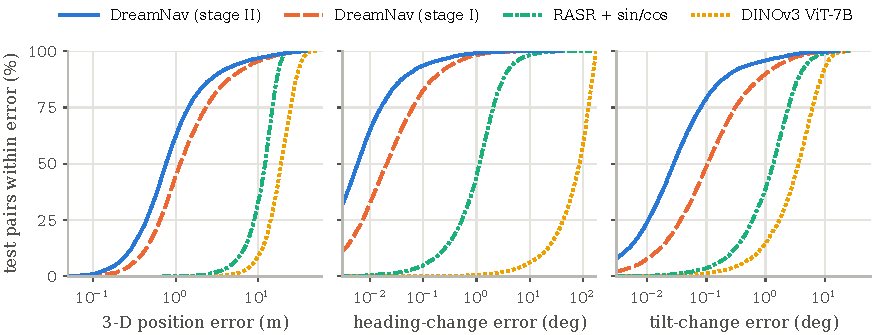
\includegraphics[width=1.0\linewidth]{figures/fig_cdf.pdf}
    \caption{<<C3>> <<C4>>}
    \label{fig:cdf}
\end{figure*}

\begin{figure}[!t]
    \centering
    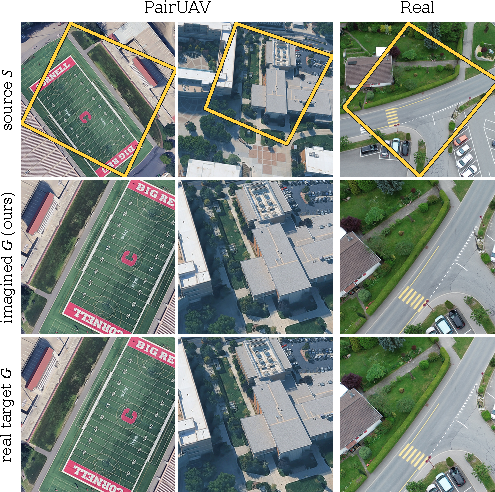
\includegraphics[width=1.0\linewidth]{figures/fig_qualitative.pdf}
    \caption{<<C18>> <<C18c>> <<C18b>> <<C19>>}
    \label{fig:qualitative}
\end{figure}

\noindent \textbf{Qualitative Results.} <<Q1>> <<Q2>>
% \noindent \textbf{定性结果。} 即使在困难的情况下，平面诱导的变换也能得到逼真的想象视图。想象视图同时还原了真实目标视图的布局和细节，能够应对高出地面的结构以及大幅度的航向和高度变化。

\subsection{Ablation Studies}

\begin{table}[!t]
  \centering
  \caption{<<C5>> <<C6>>}
  \label{tab:ablation}
  \resizebox{\columnwidth}{!}{%
    \begin{tabular}{@{}l|cccccc|c@{}}
      \toprule
      Variant & $\Delta x$ & $\Delta y$ & $\Delta z$ & $d$ & $\Delta\theta$ & $\Delta\phi$ & SR@1\,m \\
      \midrule
      RASR (MASt3R statistics)          & 7.48 & 7.47 & 2.68 & 5.14 & 5.70 & 1.87 & 11.7 \\
      + sin/cos heading regression      & 7.49 & 7.40 & 2.70 & 5.40 & 1.82 & 1.86 & 9.9 \\
      + rotation-aware two-view geometry & 7.49 & 7.40 & 1.07 & 4.80 & 0.19 & 0.64 & 12.3 \\
      + absolute heading                & 1.75 & 1.69 & 1.09 & 1.14 & 0.19 & 0.64 & 65.1 \\
      + zoom re-matching (Stage I)      & 1.37 & 1.35 & 0.81 & 0.92 & 0.12 & 0.44 & 73.1 \\
      + geometric imagination           & 1.03 & 1.02 & 0.54 & 0.68 & 0.07 & 0.20 & \textbf{83.3} \\
      + canonical-view heading (Stage II) & \textbf{0.99} & \textbf{0.98} & \textbf{0.54} & \textbf{0.68} & \textbf{0.07} & \textbf{0.20} & \textbf{83.3} \\
      \midrule
      Stage II with true absolute heading & 0.49 & 0.50 & 0.54 & 0.68 & 0.07 & 0.20 & 83.3 \\
      \bottomrule
    \end{tabular}%
  }
\end{table}

\noindent \textbf{Components of DreamNav.} <<A1>> <<A2>> <<A3>> <<A4>> <<A5>> <<A6>> <<A7>> <<A8>> <<A9>>
% \noindent \textbf{DreamNav 的各个组件。} 为了检验设计选择，我们在同一批测试样本上重复实验，但这次关注 DreamNav 的不同变体。表~\ref{tab:ablation} 的消融实验表明 DreamNav 的所有组件都有用并带来性能提升。保持 RASR 的特征不变、改用 MLP 回归航向变化的正弦和余弦时，$\mathrm{MAE}_\theta$ 从 5.70$^\circ$ 降到 1.82$^\circ$。直接运行原始匹配器只能为 47\% 的图像对解出有效的相对位姿，而在四个旋转上搜索后这一比例达到 99.3\%。没有旋转搜索时，匹配器无法匹配航向变化超过 $60^\circ$ 的图像对（见附录 I）。绝对航向未知时，世界坐标系下的位移误差停留在常数预测器的水平。放大重匹配对弱匹配的图像对尤其有效，因为受固定关键点预算的限制，整图匹配无法充分利用共视区域。在规范视图上验证航向只带来很小的提升，说明剩余的航向误差在同一地点内是系统性的，更精确的输入表示改变不了它。使用真实绝对航向可使水平误差减半，并让 DreamNav 在 $\Delta x$ 和 $\Delta y$ 上都精确到半米。

\begin{table}[!t]
  \centering
  \caption{<<C7>> <<C8>> <<C7b>>}
  \label{tab:geom}
  \small
  \setlength{\tabcolsep}{3.5pt}
  \begin{tabular}{@{}llccc@{}}
    \toprule
    \multicolumn{5}{@{}l}{all 31,273 pairs, before any fusion} \\
    Matches & Solver & $\Delta\theta$ & $\Delta\phi$ & Transl. dir. \\
    \midrule
    pass 1 & E   & 1.14 (0.033) & 2.06 (0.179) & 13.6 (1.62) \\
    pass 1 & MAP & 0.62 (0.032) & 1.11 (0.170) & 11.5 (1.57) \\
    zoom   & E   & 0.55 (\textbf{0.026}) & 1.30 (\textbf{0.133}) & 10.1 (\textbf{1.21}) \\
    zoom   & MAP & \textbf{0.37} (0.027) & \textbf{0.76} (0.135) & \textbf{8.2} (1.24) \\
    \bottomrule
  \end{tabular}
\end{table}

\begin{table}[!t]
  \centering
  \caption{<<C9>> <<C10>> <<C10b>>}
  \label{tab:imag}
  \resizebox{\columnwidth}{!}{%
    \begin{tabular}{@{}lccccc@{}}
      \toprule
      \multicolumn{6}{@{}l}{(a) raw two-view geometry on 400 pairs (errors in degrees)} \\
      Alignment before matching & Tiles & Inliers & $\Delta\theta$ & $\Delta\phi$ & Transl. dir. \\
      & & (median) & (mean) & (mean) & (median / mean) \\
      \midrule
      Zoom pass of Stage I             & 1   & 436  & 1.549 & 1.382 & 1.16 / 9.69 \\
      Rotation only, coarse pose       & 1   & 501  & 0.146 & 0.865 & 1.17 / 7.08 \\
      Plane-induced warp               & 1   & 592  & 0.095 & 0.708 & 0.90 / 6.25 \\
      Plane-induced warp               & $2{\times}2$ & 2116 & \textbf{0.073} & 0.794 & 0.50 / 5.93 \\
      Plane-induced warp (ours)        & $3{\times}3$ & \textbf{2900} & 0.111 & \textbf{0.552} & \textbf{0.41} / \textbf{3.88} \\
      \bottomrule
    \end{tabular}%
  }\\[4pt]
  \resizebox{\columnwidth}{!}{%
    \begin{tabular}{@{}lcccccc@{}}
      \toprule
      \multicolumn{7}{@{}l}{(b) refined fusion on 3,000 test pairs (MAE)} \\
      Variant & $\Delta\theta$ ($^\circ$) & $\Delta\phi$ ($^\circ$) & $d$ (m) & $\Delta z$ (m) & $\ell_x$ (m) & $\ell_y$ (m) \\
      \midrule
      Stage I                          & 0.132 & 0.405 & 0.913 & 0.770 & 0.797 & 0.911 \\
      Refined fusion w/o imagined matches & 0.134 & 0.412 & 0.931 & 0.789 & 0.817 & 0.928 \\
      Refined fusion w/o verification  & \textbf{0.072} & 0.192 & 0.664 & \textbf{0.544} & 0.468 & 0.487 \\
      Refined fusion (ours)            & \textbf{0.072} & \textbf{0.188} & \textbf{0.661} & 0.545 & \textbf{0.455} & \textbf{0.486} \\
      \bottomrule
    \end{tabular}%
  }\\[4pt]
  % (c) The diffusion row is copied from diffusion_results.jpg; that file does not record the number of test pairs.
  \resizebox{\columnwidth}{!}{%
    \begin{tabular}{@{}lccccc@{}}
      \toprule
      \multicolumn{6}{@{}l}{(c) source of the imagined view (MAE)} \\
      Variant & $\Delta x$ (m) & $\Delta y$ (m) & $\Delta z$ (m) & $\Delta\theta$ ($^\circ$) & $\Delta\phi$ ($^\circ$) \\
      \midrule
      Stage I (no imagination)         & 1.37 & 1.35 & 0.81 & 0.12 & 0.44 \\
      Diffusion retrieval              & 1.96 & 1.87 & 1.43 & 0.43 & 0.65 \\
      Geometric imagination (ours)     & \textbf{0.99} & \textbf{0.98} & \textbf{0.54} & \textbf{0.07} & \textbf{0.20} \\
      \bottomrule
    \end{tabular}%
  }
\end{table}

\noindent \textbf{Imagination-Refined Stage.} <<G1>> <<G2>> <<G3>> <<G4>> <<G5>> <<G6>> <<G7>> <<G8>> <<G9>> <<G10>> <<G11>> <<G12>>
% \noindent \textbf{想象精修阶段。} 我们渲染想象视图，并把每对图像的图块数从 $1$ 变到 $3{\times}3$（见表~\ref{tab:imag}a）。不出所料，图块越多越好；只用一个图块时匹配器的关键点常常“不够用”，内点数少到五分之一。用粗估计位姿重新对齐、把纯旋转变换换成平面诱导的单应、在原始分辨率上分块匹配，这三步都对精修相对于粗估计阶段 zoom pass 的提升有贡献。这一提升并不是多加一层回归器带来的：对照实验表明，同样的回归器如果不给想象匹配，相对粗估计阶段没有任何增益，误差还略有上升（表~\ref{tab:imag}b）。去掉验证分数后 DreamNav 仍能有效精修，性能只有很小的下降（$\ell_x$ 从 0.455\,m 到 0.468\,m）。我们还考察了多轮迭代带来的精度变化：想象视图与真实视图之间的位移（一个不需要标签、反映引导位姿精度的量）在粗估计阶段之后是 7.6 像素，经过一轮精修后是 5.0 像素。注意第二轮在平移方向中位误差上的增益（0.03$^\circ$）远小于 zoom pass 与第一轮之间的差距（0.75$^\circ$）。我们还把几何想象换成基于扩散模型的检索：对粗估计附近的候选位姿，用扩散模型合成视图，再与目标视图比较，以此代替平面诱导变换和匹配。在同样的粗估计之上做这一替换，每个位姿参数的误差都显著上升，$\mathrm{MAE}_\theta$ 从 0.12$^\circ$ 升到 0.43$^\circ$（表~\ref{tab:imag}c）。我们认为这一退化的原因在于使用了合成视图并在候选位姿中做检索：这放弃了像素级几何，并把估计限制在采样到的候选位姿上。

\subsection{Analysis}

\begin{figure*}[!t]
    \centering
    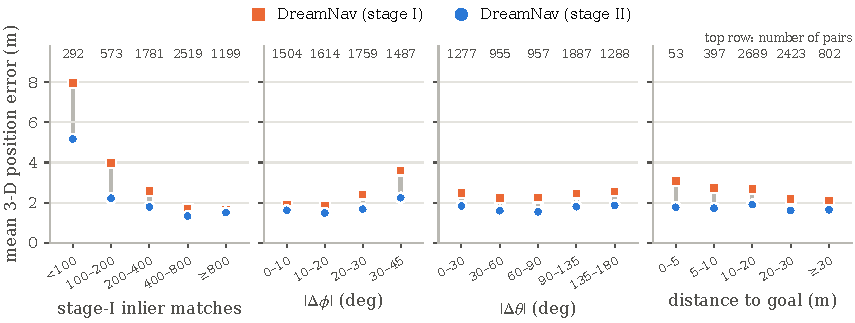
\includegraphics[width=1.0\linewidth]{figures/fig_breakdown.pdf}
    \caption{<<C11>> <<C12>>}
    \label{fig:breakdown}
\end{figure*}

\noindent \textbf{Where Does the Refinement Help?} <<N1>> <<N2>> <<N3>> <<N4>> <<N5>> <<N6>>
% \noindent \textbf{精修在哪些样本上起作用？} 图~\ref{fig:breakdown} 考察两个阶段（粗估计与精修）在不同内点数、旋转和距离区间的测试样本上的效果。提升在所有区间上都是一致的，无论按旋转还是按距离划分。对中等难度的样本（例如粗估计内点数为 100--200 的图像对），精修找回了多得多的对应点，位置误差几乎减半，从 3.98\,m 降到 2.21\,m。在视觉重叠很小的情况下（例如内点少于 100），精修需要更多的对应点才能成功。评测之后，我们对 290 个测试地点重采样 1,000 次，给出 95\% 置信区间。精修阶段更稳定地到达目标：成功率高 10.2 个百分点（区间 9.1--11.3），平均位置误差低 0.68\,m（0.61--0.74）。

\begin{figure}[!t]
    \centering
    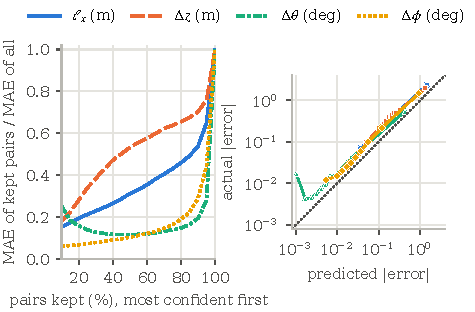
\includegraphics[width=1.0\linewidth]{figures/fig_reliability.pdf}
    \caption{<<C13>> <<C14>>}
    \label{fig:reliability}
\end{figure}

\noindent \textbf{Reliability of the Predicted Error.} <<V0>> <<V1>> <<V2>> <<V3>> <<V4>> <<V5>> <<V6>> <<V7>>
% \noindent \textbf{预测误差是否可靠。} 本小节考察“为每个候选估计预测误差”这一做法是否有效。具体而言，我们想量化融合中用作权重的误差预测的质量，并分析它们刻画了什么。首先，图~\ref{fig:reliability}（左）给出四个位姿参数的稀疏化曲线，展示了去掉预测误差高于各百分位阈值的图像对后模型性能如何提升。只保留最有把握的一半时，测试样本上俯仰变化的平均误差从 0.20$^\circ$ 降到 0.02$^\circ$。其次，图~\ref{fig:reliability}（右）用测试集上的校准曲线分析误差预测的质量；误差预测越好，校准曲线越接近直线 $y=x$。不过预测误差比实际误差低一个近似恒定的倍数（1.5--2 倍），这主要是因为回归目标取了平方根：在这种凹变换之后做拟合，回归器无法恢复偏态分布的均值。

\noindent \textbf{Limitations.} <<L1>> <<L2>> <<L3>>
% \noindent \textbf{局限。} 当两个视图几乎不重叠，或场景缺少关于绝对航向的线索时，位姿估计是困难的。在 DreamNav 位置误差超过 1\,m 的 2,422 个样本中，44\% 仅仅由绝对航向误差造成，17\% 是因为粗估计内点少于 200，39\% 来自尺度和平移方向的其余误差。DreamNav 在南半球的地点也会失败（阴影方向相反），并且对飞行高度的变化更敏感。

\subsection{Zero-Shot Transfer to Real Drone Photographs}
\label{sec:real}

<<T1>> <<T2>>
% 前面的实验精确地量化了 DreamNav 的精度，但其中不包含传感器、飞行高度或成像方式的任何变化。因此我们转向真实的无人机照片，在零样本设定下评估几何想象的收益。

\noindent \textbf{Dataset.} <<T3>> <<T4>> <<T5>> <<T6>>
% \noindent \textbf{数据集。} 我们用 M\'ezi\`eres 数据集考察真实飞行中的位姿估计，指标与第~\ref{sec:setup} 节相同。图像由一架在村庄上空 60\,m 飞行的 DJI Phantom 4 RTK 拍摄，位姿真值来自 RTK 和光束法平差。我们只使用相机间距不超过 30\,m 的照片对，从中采样 600 对用于评测。采样时按“基线/高度”比对难度做了均衡。

\noindent \textbf{Setup.} <<T7>> <<T8>> <<T9>>
% \noindent \textbf{设置。} 我们对照片去畸变并重采样，使其内参与 PairUAV 的标定 $\mathbf{K}$ 一致。需要强调，所有结果都由\emph{同一个} DreamNav 模型得到（唯一与场地有关的输入是飞机自身报告的飞行高度，用它对估计位移做缩放），即我们从未在真实照片上微调模型。位置误差在源相机的水平坐标系中计算，因为绝对航向无法从渲染图像的阴影迁移到真实阴影。

\begin{table*}[!t]
    \centering
    \caption{<<C15>> <<C16>> <<C16b>>}
    \label{tab:real}
    \small
    \setlength{\tabcolsep}{3.5pt}
    \begin{tabular}{@{}l|ccccc|ccccc@{}}
    \toprule
    & \multicolumn{5}{c|}{Within training range (300 pairs)} & \multicolumn{5}{c}{Beyond training range (300 pairs)} \\
    Methods & Pos. (m) & SR@1\,m & SR@2\,m & $\Delta\phi$ & Dir. & Pos. (m) & SR@1\,m & SR@2\,m & $\Delta\phi$ & Dir. \\
    \midrule
    Constant (zero motion)       & 7.84  & 1.3  & 3.7  & \textbf{0.45} & 90.0 & 21.71 & 0.0 & 0.0 & \textbf{0.55} & 90.0 \\
    RASR + sin/cos               & 11.42 & 5.7  & 11.0 & 3.40 & 41.0 & 23.54 & 3.0 & 5.0 & 7.27 & 55.5 \\
    RASR + sin/cos, rescaled     & 5.10  & 18.3 & 34.3 & 3.40 & 41.0 & 18.88 & 0.0 & 2.0 & 7.27 & 55.5 \\
    \midrule
    Ours (Stage II), no flight height & 16.42 & 2.0 & 3.7 & 1.62 & \textbf{1.9} & 24.13 & 1.0 & 2.3 & 4.94 & \textbf{45.5} \\
    Ours (Stage I)               & 1.43  & 45.0 & 69.3 & 1.90 & 4.4  & 18.27 & 0.0 & 7.3 & 5.12 & 48.1 \\
    Ours (Stage II)              & \textbf{0.84} & \textbf{63.3} & \textbf{80.3} & 1.62 & \textbf{1.9} & \textbf{18.03} & \textbf{5.0} & \textbf{11.0} & 4.94 & \textbf{45.5} \\
    \bottomrule
    \end{tabular}
\end{table*}

\begin{figure}[!t]
    \centering
    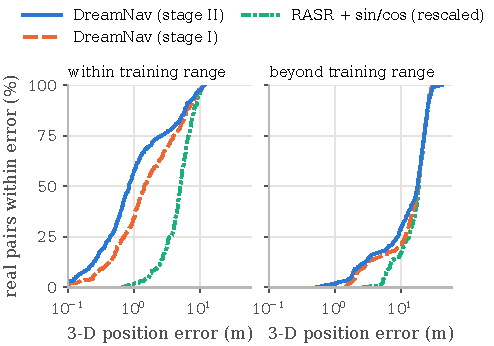
\includegraphics[width=1.0\linewidth]{figures/fig_real.pdf}
    \caption{<<C17>>}
    \label{fig:real}
\end{figure}

\noindent \textbf{Results.} <<T10>> <<T10b>> <<T11>> <<T12>> <<T13>> <<T14>> <<T15>> <<T16>>
% \noindent \textbf{结果。} 表~\ref{tab:real} 表明，在“基线/高度”比的两个区间内，DreamNav 在所有指标上都优于全部回归基线。不过在俯仰变化上看不到提升，常数预测器在这一项上更准，因为这些照片之间云台几乎不动。在训练范围内 DreamNav 是准确的，尽管它只在渲染图像上训练过。精修在真实照片上同样提高了所有阈值下的成功率，而真实照片的视差更强，这对平面诱导的变换是不利条件。这说明只需平面诱导的变换，想象就能带来收益，而且尽管融合只在渲染图像对上拟合，它仍能很好地泛化。然而超出训练范围后性能显著下降（成功率 5.0\%），说明低空宽基线仍然困难，需要进一步研究。与相对几何不同，DreamNav 的尺度恢复假设飞行高度与训练时一致。这一假设不成立时系统就会失败：不提供飞机报告的飞行高度时，成功率从 63.3\% 降到 2.0\%。

\subsection{Closed-Loop Navigation}
\label{sec:closedloop}

\noindent \textbf{Setup.} <<S1>> <<S2>> <<S3>> <<S4>> <<S5>> <<S6>> <<S7>> <<S7b>> <<S8>> <<S8b>> <<S9>> <<S10b>>
% \noindent \textbf{设置。} 接下来介绍衡量 DreamNav 闭环导航能力的实验。为此，我们在 8 个留出的测试地点上评估“以图像为目标”的导航任务。首先用每个地点 150 张图像中的 135 张（位姿和内参已知），借助 gsplat 重建一个 3D 高斯泼溅模型。对每个地点 10 张留出的目标图像，各从其余相机中采样 2 个起始位姿，渲染无人机当前看到的视图，并带执行噪声地执行估计出的位姿变化。这些观测是在原始分辨率下从泼溅模型采样渲染得到的，与作为目标的真实图像相互独立。每条指令都被随机扰动：长度的 3\% 加每轴 5\,cm，航向 $0.2^\circ$，俯仰 $0.1^\circ$。我们比较 DreamNav 的两个变体（带与不带想象精修阶段），以考察想象的作用。闭环评测时精修阶段启用其近距离模式（第~\ref{sec:servo} 节），前面的实验则没有启用。只要策略自己估计的到目标距离仍高于阈值 $\tau$，就允许它继续飞行，最多 5 步。阈值取得更小可以让无人机离目标更近，但也增加了在比训练时更短的基线上行动的风险。评价指标包括停止时的位置误差、飞行的步数，以及最终落在目标 1\,m 以内的回合比例。不过 DreamNav 在渲染视图上要差一些：渲染图的纹理明显更模糊，估计也因此更粗（同一批图像对上 $\ell_x$ 的中位误差为 0.48\,m，真实图像为 0.36\,m）。

\noindent \textbf{Results.} <<S10>> <<S11>> <<S12>> <<S13>> <<S14>> <<S14b>> <<S15>> <<S16>> <<S17>> <<S18>>
% \noindent \textbf{结果。} 结果汇总于表~\ref{tab:nav}。只执行一步时，两个变体都能走完初始距离的绝大部分，其中精修估计的中位误差最低（从 18.9\,m 出发，剩 1.32\,m）。闭环之后，完整模型的成功率从 38.8\% 提高到 81\% 以上，平均只需 2.2 步。在 $\tau = 1$\,m 时，完整模型的成功率比只用粗估计阶段高 25 个百分点，说明近距离模式是有效的。完整模型总体上比粗估计阶段更成功，但并不是在扫描的每一个阈值上都更成功（图~\ref{fig:nav}）。阈值较大时粗估计阶段同样成功，因为此时完整模型在一半以上的回合里走完第一步就停了，近距离模式还来不及起作用；阈值较小时它才有足够的步数发挥作用。一个假设是，融合模型对短于 5\,m 的基线外推能力差，而这类样本在其训练对中不到 1\%。例如在距目标 0.5\,m 到 1\,m 时，粗估计阶段把剩余距离高估到中位数 1.34\,m，而近距离模式估计为 0.78\,m。我们报告了四个阈值（表~\ref{tab:nav}），发现近距离模式提高了导航性能，其中不超过 1.25\,m 的阈值效果更好。完整模型总是更快满足停止条件：$\tau = 1$\,m 时平均 2.2 步，粗估计阶段是 3.8 步。

\begin{table*}[!t]
    \centering
    \caption{<<C20>>}
    \label{tab:nav}
    \small
    \setlength{\tabcolsep}{4.5pt}
    \begin{tabular}{@{}l|cc|ccc|ccc|ccc|ccc@{}}
    \toprule
    & \multicolumn{2}{c|}{One step} & \multicolumn{3}{c|}{$\tau = 0.5$\,m} & \multicolumn{3}{c|}{$\tau = 1$\,m} & \multicolumn{3}{c|}{$\tau = 1.5$\,m} & \multicolumn{3}{c}{$\tau = 2$\,m} \\
    Variant & Err. & SR & Steps & Err. & SR & Steps & Err. & SR & Steps & Err. & SR & Steps & Err. & SR \\
    \midrule
    Ours (Stage I)  & 1.41 & 37.5 & 4.85 & 1.44 & 30.0 & 3.76 & 0.83 & 56.9 & 2.77 & 0.72 & 70.0 & 2.21 & \textbf{0.73} & \textbf{70.6} \\
    Ours (Stage II) & \textbf{1.32} & \textbf{38.8} & \textbf{3.82} & \textbf{0.63} & \textbf{66.9} & \textbf{2.23} & \textbf{0.56} & \textbf{81.9} & \textbf{1.78} & \textbf{0.69} & \textbf{73.1} & \textbf{1.62} & \textbf{0.73} & 67.5 \\
    \bottomrule
    \end{tabular}
\end{table*}

\begin{figure}[!t]
    \centering
    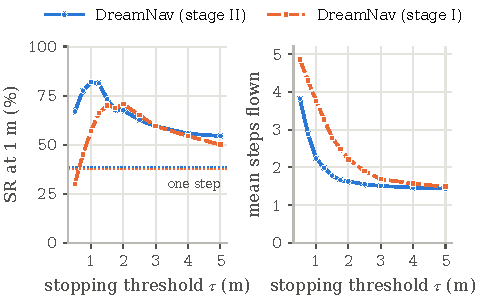
\includegraphics[width=1.0\linewidth]{figures/fig_nav.pdf}
    \caption{<<C21>>}
    \label{fig:nav}
\end{figure}
